\documentclass{VUMIFPSkursinis}
\usepackage{algorithmicx}
\usepackage{algorithm}
\usepackage{algpseudocode}
\usepackage{amsfonts}
\usepackage{amsmath}
\usepackage{bm}
\usepackage{caption}
\usepackage{color}
\usepackage{float}
\usepackage{graphicx}
\usepackage{listings}
\usepackage{float}
\usepackage{subfig}
\usepackage{wrapfig}
\usepackage[hidelinks]{hyperref}
\usepackage{todonotes}

% Titulinio aprašas
\university{Vilniaus universitetas}
\faculty{Matematikos ir informatikos fakultetas}
\department{Programų sistemų katedra}
\papertype{Programų kūrimo proceso laboratorinis darbas}
\title{Įmonės ,,Mėnuliukų technologijos" programų kūrimo proceso aprašas (Pirmas laboratorinis darbas)}
\titleineng{Description of the development process of the ,,Moon Technologies" company (First laboratory work)}
\status{4 kurso 3 grupės studentai}
\author{Matas Savickis, Justas Tvarijonas, Džiugas Mažulis}
\secondauthor{Greta Pyrantaitė, Andrius Bentkus}


\supervisor{Saulius Ragaišis, Doc., Dr.}
\date{Vilnius – \the\year}

% Nustatymai
% \setmainfont{Palemonas}   % Pakeisti teksto šriftą į Palemonas (turi būti įdiegtas sistemoje)
\bibliography{bibliografija}

\begin{document}
\maketitle

\tableofcontents

\sectionnonum{Įvadas}
	Šiame darbe bus pristatytas ,,Mėnuliukų technologijų" programų kūrimo procesas.
	Pats procesas yra paremtas Agile metodologija su minimaliais pakeitimais reikalavimų rinkime.
	Proceso pradžioje stengiamės su užsakovu išsiaiškinti norimus įgyvendinti funkcionalumus ir bendraujant kartu su užsakovu sudaryti reikalavimus. 
	Sudarant reikalavimus yra diskutuojama ir sistemos ateities vizija, siekiant susidaryti geresnę perspektyvą sistemos ateičiai ir darbartiniams reikalavimams.
	Įmonė įvertina, kiek valandų užtruks kiekvieno funkcionalumo sukūrimas, o mokestis yra imamas už pradirbtas valandas.
	Klientui nesutikus su pateiktomis kainomis yra daromi susitikimai siekiant paaiškinti valandų vertinimą. Po susitikimų funkcionalumo įgyvendinimo valandos gali keistis, arba funkcionalumas bus atsisakytas. 
	Kiekvieno sprinto pradžioje, po reikalavimų pasitikslinimo, yra sudaromi priėmimo testai, kuriuos praėjus kliento prašoma susimokėti už atliktus darbus.

\section{Kūrimo procesas}
	\begin{figure}[htbp]
	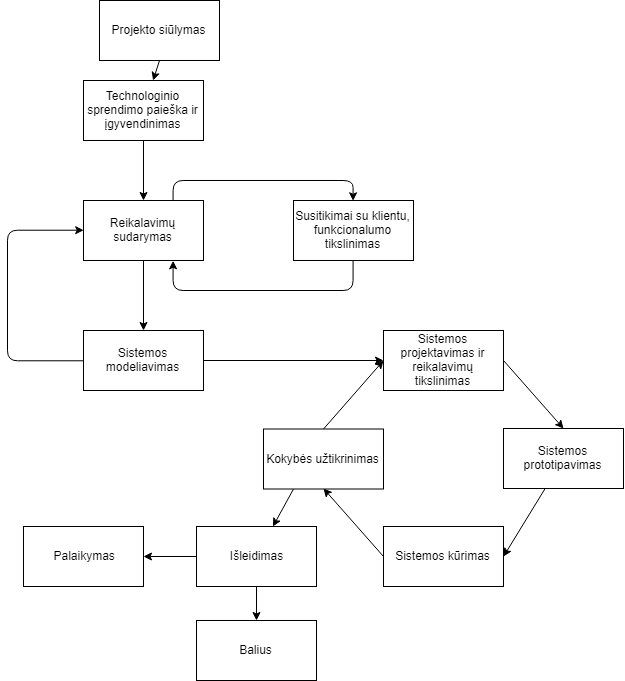
\includegraphics[scale=0.6]{img/SoftwareProcessMoonTechnologies}
	\caption{Sistemos kūrimo procesas} % Antraštė įterpiama po paveikslėlio
	\label{img:kurimoProcesas}
	\end{figure}
	\subsection{Projekto siūlymas}

	\begin{center}
		\begin{table}[ht]
			\caption{Projekto siūlymo procesas}
		\begin{tabular}{ | l | l | } 
		\hline
	Pavadinimas:         & Projekto siūlymas.                                      \\ \hline
	Tikslas: 	           & Aptarti galimą projektą su galimu klientu. 							\\ \hline
	Vykdytojai:          & Projekto vadovas ir klientas.                             \\ \hline
	Veiklos:             & V1 - Aptariama sistemos aprėptis. 													\\
											 & V2 - Nustatomos kainos ribos iki pirmo sistemos išleidimo.  \\
											 & V3 - Pirminės sutarties pasirašymas .													\\ \hline
	Naudojami produktai: & NP1 - Buvusių projektų dokumentai. 													 \\ \hline
	Sukuriami produktai: & SP1 - Pirminė sutartis sistemos projektavimui. 								\\ \hline
\end{tabular}
\end{table}
\end{center}
\begin{enumerate}
	\item Pirmas susitikimas, kuriame aptariamas galimas projektas, kiekviena pusė išsako savo lūkesčius, pasidalinama įdėjomis.
	\item Po susitikimo įmonė paruošia pradininį pasiūlymą, į kurį įeina orientacinės finansų ribos, žmonių ištekliai, kurie galėtų būtų skiriami šiam projektui. Šis pasiūlymas aptariamas su klientu, kartu su juo dokumentuojami funkcionalumai, kurių klientas nori pirmame sistemos išleidime. Sėkmingai tesiantis tolesnėms deryboms nutariama dėl pradinio technologinio sprendimo pasiūlymo datos, bei finansavimo jam.
	\item Pasirašoma pradinė sutartis, kurioje dokumentuojama prieš tai aptarta informacija. Ši sutartis galioja iki pirmojo prototipo pasiūlymo, po kurio atnaujinamos derybos dėl tolesnio projekto vystymosi.
\end{enumerate}
	\subsection{Technologinio sprendimo paieška ir įgyvendinimas}
		\begin{center}
			\begin{table}[ht]
				\caption{Technologinio sprendimo paieškos ir įgyvendinimo procesas.}
					\begin{tabular}{ | l | l | } 
						\hline
							Pavadinimas:         & Technologinio sprendimo paieška ir įgyvendinimas.                                      \\ \hline
							Tikslas: 	           & Išskirti technologijas ir jų versijas, kurios bus naudojamos projekte. 							\\ \hline
							Vykdytojai:          & Projekto vadovas, klientas, programuotojas.                             \\ \hline
							Veiklos:             & V1 - Aptarti technologijas, šiuo metu naudojamas projekte. 													\\
											 & V2 - Nustatomos technologijų kainos, kurios bus naudojamos projekte. \\
											 & V3 - Nutariama dėl technologinių alternatyvų.													\\ \hline
							Naudojami produktai: & NP1 - Esamos sistemos dokumentacija, norimų naudoti technologijų \\& dokumentacija ir kainynas. 													 \\ \hline
							Sukuriami produktai: & SP1 - Technologinių sprendimų ir jų alternatyvų dokumentas su \\& preliminariomis technologijų licenzijų kainomis. 								\\ \hline
					\end{tabular}
			\end{table}
		\end{center}

\begin{enumerate}
	\item{Aptariamos technologijos, kurios šiuo metu naudojamos projekte - išskiriami technologiniai karkasai, duomenų bazės, programavimo kalbų versijos ir kitos naudojamos technologijos ir jų versijos.
	Įvertinamas esamų technologijų saugumo lygis, greitaveika ir ateities palaikymas. 
	Pasiūlomi technologiniai sprendimai pagrindžiant jų naudą sistemai.}
	\item{Nustatomos technologijų kainos, kurios bus naudojamos projekte - paskaičiuojamos dabartinių technologijų kainos ir naujų siūlomų technologijų kainos.}
	\item{Nutariama dėl technologinių alternatyvų - jeigu įmanoma klientui pasiūlomi atviro kodo technologiniai sprendimai siekiant sutaupyti pinigų. 
		Pateikiamas palyginimas tarp dabartinės sistemos technologijos, siūlomos technologijos ir atviro kodo technologijų sprendimų. }
\end{enumerate}

	\subsection{Reikalavimų ciklas}
		\begin{center}
			\begin{table}[ht]
				\caption{Reikalavimų ciklo procesas.}
					\begin{tabular}{ | l | l | } 
						\hline
							Pavadinimas:         & Reikalavimų ciklas.                                      \\ \hline
							Tikslas: 	           & Suformuoti funkcinius ir nefunkcinius reikalavimus.							\\ \hline
							Vykdytojai:          & Programuotojas, analistas, klientas.                            \\ \hline
							Veiklos:             & V1 - Iš kliento pateiktų verslo reikalavimų suformuojame funkcinius \\ & reikalavimus. 													\\
											 & V2 - Pristatome klientui sudarytus funkcinius reikalavimus ir tiksliname \\& pateiktus verslo reikalavimus. \\
											 & V3 - Siūlomi nefunkciniai reikalavimai.												\\ \hline
							Naudojami produktai: & NP1 - Kliento pateiktas verslo reikalavimų dokumentas.													 \\ \hline
							Sukuriami produktai: & SP1 - Funkcinių ir nefunkcinių reikalavimų dokumentas.								\\ \hline
					\end{tabular}
			\end{table}
		\end{center}

\begin{enumerate}
	\item{Iš kliento pateiktų verslo reikalavimų suformuojame funkcinius reikalavimus - mūsų įmonės verslo analitikas dirbdamas kartu su programuotojais suformuoja atsekamus (su indentifikacijos kodu) funkcinius reikalavimus.}
	\item{Pristatome klientui sudarytus funkcinius reikalavimus ir tiksliname pateiktus verslo reikalavimus - suformavus funkcinius reikalavimus planuojami susitikimai su klientu, siekiant jam pristatyti suformuotus reikalavimus, patikslinti pateiktus verslo reikalavimus ir toliau tikslinti reikalavimus iki kol reikalavimai tenkis klientą ir bus suprantami programuotojų komandai, kuri dirbs prie kliento projekto.}
	\item{Siūlomi nefunkciniai reikalavimai - jeigu klientas pats nepateikė nefunkcinių reikalavimų įmonė pati pateikia nefunkcinių reikalavimų siūlymus pagal esamo projekto apimtį ir biudžetą. Pateikti nefunkciniai reikalavimai yra aptariami ir tikslinami su klientu.}
\end{enumerate}
		
	\subsection{Sistemos modeliavimas}
	\begin{center}
		\begin{table}[ht]
			\caption{Sistemos modeliavimo procesas}
		\begin{tabular}{ | l | l | } 
		\hline
	Pavadinimas:         & Sistemos modeliavimas.          		 					 \\ \hline
	Tikslas: 	           & Skurti pradinę sistemos versiją. 																	\\ \hline
	Vykdytojai:          & Programuotojas, analistas.  \\ \hline
	Veiklos:             & V1 - Reikalavimų analizė iš implementacijos pusės. 		          \\
											 & V2 - Pradinės sistemos rašimas ir testavimas.					             \\
											 & V3 - Atnaujintos sutarties pasirašymas.									          \\ \hline
	Naudojami produktai: & NP1 - Sistemos reikalavimai. 													  \\
											 & NP2 - Architektūrinių sprendimų dokumentas. \\ \hline
	Sukuriami produktai: & SP1 - Pradinė kodo bazė. 																	          \\
											 & SP2 - Atnaujinta projekto sutartis.										           \\ \hline
\end{tabular}
\end{table}
\end{center}

\begin{enumerate} 
	\item Pagal gautus reikalavimus programuotojų komanda sumodeliuoja pradinės sistemos implementaciją, pradedama rašyti kodo bazė ant kuriuos ateinančiuose sprintuose bus statoma visa sistema.
	\item Sukurtas sistemos modelis yra pristatomas klientui, jeigu jį tenkina pasirinkta kryptis, yra pasirašoma sutartis tolimesniam bendradarbiavimui.
\end{enumerate}
		
	\subsection{Sprintas}
	Sprintu skaitome dvi savaites, kurių pabaigoje yra įvykdytas verslo analitiko ar komandos parinktas užduočių skaičius ir matomas apčiuopiamas rezultatas - veikiantis funkcionalumas. Sprinto ilgis - 2 savaitės - pasirinktas taip, kad nebūtų sunku numatyti ir suplanuoti užduočių tam laiko tarpui ir taip, kad būtų pakankamai laiko jas įvykdyti iki galo. Sprintas turi kelias veiklas, kurios skirtos palaikyti efektyvią programos kūrimo eigą ir užtikrinti, kad rezultatas būtų pasiektas laiku.
	\subsubsection{Sprinto užduočių tikslinimas ir vertinimas}
	\begin{center}
		\begin{table}[ht]
			\caption{Sprinto užduočių tikslinimo ir vertinimo procesas}
		\begin{tabular}{ | l | l | } 
		\hline
	Pavadinimas:         & Sprinto užduočių tikslinimas ir vertinimas.          		 					 \\ \hline
	Tikslas: 	           & Įvertinti ir paanalizuoti užduotis. 																	\\ \hline
	Vykdytojai:          & Programuotojas bei Įmonės analistas arba užsakovo atstovas, klientas  \\ \hline
	Veiklos:             & V1 - Analistas paaiškina užduotis iš verslo perspektyvos. 		          \\
											 & V2 - Užduočių vertinimo sesija tarp programuotojų.					             \\
											 & V3 - Įvertintų užduočių aptarimas su analistu 									          \\ \hline
	Naudojami produktai: & NP1 - Užduočių sąrašas. 													 							           \\ \hline
	Sukuriami produktai: & SP1 - Sprinto užduočių sąrašas. 																	          \\ 
											 & SP2 - Įvertintos užduotys backloge(vertimas?) 										           \\ \hline
\end{tabular}
\end{table}
\end{center}
\begin{enumerate}
	\item Pradinis užduočių aptarimas su analistu arba užsakovo atstovu, šiame aptarime paaiškinami kiekvienos užduoties scenarijai iš dalykinės srities pusės, paaiškinami reikalavimai, kurie turi būti įgyvendinami prieš pabaigiant užduotį. Diskusijos su programuotojais metu galimi užduočių ar jų priėmimo kriterijų pakeitimai arba, jeigu jų negalima atlikti nepasitarus su klientu, užduotis yra atnaujinama vėliau, pasitarus su klientu.
	\item Atlikus pradinį aptarimą kartu su analistu arba verslo atstovu rengiama diskusija tarp programuotojų, kuriame kiekviena užduotis yra įvertinama taškais, vertinama fibonačio sekos skaičiais, o skaičiaus reikšmė yra viena programuotojo darbo diena. Šioje diskusijoje programuotojai diskutuoja apie galimą kiekvienos užduoties implementaciją, bei jos sudėtingumą, tada balsuojama dėl šiai užduočiai skiriamo balų skaičiaus. Taip aptariamos visos dar neįvertintos užduodys, tuo atvėju, jeigu gilinantis į implementaciją atsiranda neaiškumų dėl dalykinės srities, užduotis yra blokuojama paliekant komentarą, kad jį radęs analistas galėtų patikslinti užduotį.
	\item Atlikus užduočių vertinimą analistas arba verslo atstovas sudeda sekančio sprinto struktūra pagal galimą talpą (talpa lygi programuotojų skaičiui padauginta iš 8). 
\end{enumerate}
	\subsubsection{Užduočių analizė}
	\begin{center}
		\begin{table}[ht]
		\caption{Uzduociu analizė}
		\begin{tabular}{ | l | l | } 
		\hline
		Pavadinimas:         & Užduočių analizė                               \\ \hline
		Tikslas: 	           & Surinkti visą reikalingą informaciją užduočiai įvykdyti\\ \hline
		Vykdytojai:          & Programuotojas                          \\ \hline
		Veiklos:             & V1 - Klausimų, į kuriuos reikia atsakymo, iškėlimas												\\ 
						             & V2 - Informacijos rinkimas, atsakymas į klausimus\\ 
					 	             & V3 - Įgyvendinimo alternatyvų aprašymas\\
					 	             & V4 - Jei reikia, įrodymas, kad alternatyva veiks ar neveiks							 \\ \hline
		Naudojami produktai: & NP1 - Užduočių sąrašas 																																															 \\ \hline
		Sukuriami produktai: & SP1 - Atsakymai į iškeltus klausimus\\
								& SP2 - Implementacijos alternatyvų sąrašas ir aprašymas \\
								& SP3 - Jei reikia, pasirinktos alternatyvos supaprastinta implementacija\\ 
								& SP4 - Jei reikia, papildytas, patobulintas užduočių sarašas\\\hline
		\end{tabular}
	\end{table}
		\end{center}
	Turint pilnai aprašytas užduotis vyksta užduočių analizė, jei yra tam poreikis. Jei kyla daugiau neiškumų dėl projekto vykdymo ateities planų gali būti sukuriamos atskiros užduoties tam tikros srities išsiaiškinimui tam, kad geriau išsiaiškinti galimas implementacijos alternatyvas. Tokios analizės rezultatas - dokumentas, pateikiantis klausimus ir atsakymus, implementacijos alternatyvas ir kilusius kitus pastebėjimus. Po analizės turi būti aišku, kaip ir su kokiomis technologijomis užduotis bus įvykdoma ir, jei reikalinga, tikslinamos užduotys. 
	\par Jei analizė reikalinga mažesniu mastu, bet dar negalima iškart imti ir programuoti - asmeniškai, jau pasiėmus užduotį, aiškinamasi, kokių žinių trūksta ir kas jas galėtų suteikti. Tai gali būt pasikalbėjimas su kolegomis ar panašių užduočių implementacijos pavyzdžių ieškojimas. Šios veiklos pabaigoje jau galima pradėti progamuoti.
	\subsubsection{Programavimas}
	\begin{center}
		\begin{table}[ht]
		\caption{Programavimo procesas}
		\begin{tabular}{ | l | l | } 
		\hline
		Pavadinimas:         & Programavimas.                      \\ \hline
		Tikslas: 	           & Suprogramuoti sprinto užduotis.      \\ \hline
		Vykdytojai:          & Programuotojai.                       \\ \hline
		Veiklos:             & V1 - Kodo rašymas. 									  \\
						             & V2 - Rankinis testavimas. 							 \\
					 	             & V3 - Automatinių testų rašymas. 					\\ \hline
		Naudojami produktai: & NP1 - Užduočių aprašymas.								 \\ \hline
		Sukuriami produktai: & SP1 - Užduoties kodas. 							  		\\
												 & SP2 - Modulių testai. 											 \\
												 & SP3 - Integraciniai testai. 									\\ \hline
		\end{tabular}
	\end{table}
		\end{center}
		\begin{enumerate}
			\item Atlikus užduočių analizę ir išsiaiškinus kodo implementacijos kryptį, pradedama rašyti užduoties implementacija. Atlikus implementaciją kodas yra peržiūrymas komandus narių, bet pagal jų rekomendacijas pamodifikuojamas.
			\item Atlikus užuodoties implementaciją programuotojas iš pradžių rankiniu būdu pratestuoja ar jo sukurtas funkcionalumas veikia tinkamai, o radęs netikslumų juos ištaiso.
			\item Rankinio testavimo būdu pratestavus funkcionaluma yra rašomi automatiniai testai skirti patikrinti sudėtingesnius scenarijus, bei ateities regresiniam testavimui užtikrinti. Į šiuos testus įeina modulių, aptarnavimo bei integraciniai testai.
		\end{enumerate}
	Šis žingsnis glaudžiai susijęs su prieš jį einančiomis fazėmis, jame vykdomas suprojektuotos sistemos dalies įgyvendinimas, kuris apima kodo rašymą, automatizuotų testų kūrimą, konfigūracijos pakeitimus ir duombazės kūrimą. Ši fazė įgyvendinama tik gerai išsiaiškinus ir susidokumentavus reikalavimus ir jau turint prototipą, kad kuriama programa atitiktų kliento lūkesčius ir reikalingų pakeitimų būtų mažiau.
	\subsubsection{Priėmimo testavimas}
	\begin{center}
		\begin{table}[ht]
		\caption{Priėmimo testavimo procesas}
		\begin{tabular}{ | l | l | } 
		\hline
		Pavadinimas:         & Priėmimo testavimas                                       \\ \hline
		Tikslas: 	           & Patikrinti ar sistema atitinka verslo reikalavimus \\ \hline
		Vykdytojai:          & Analistas ir programuotojai                                \\ \hline
		Veiklos:             & V1 - Priėmimo testavimo planavimas													\\
						             & V2 - Priėmimo testų klasifikavimas					 \\
					 	             & V3 - Priėmimo testavimas 														\\ \hline
		Naudojami produktai: & NP1 - Verslo reikalavimų dokumentas 																				\\ \hline
		Sukuriami produktai: & SP1 - Priėmimo testų planas 																								\\
												 & SP2 - Priėmimo testai																	 \\ \hline
		\end{tabular}
	\end{table}
		\end{center}
	Priėmimo testavimo procesas vykdomas cikliškai su programavimo procesu kiekviename sprinte. Proceso metu, prieš sukurtos sistemos ar jos dalies pristatymą klientui, tikrinama, ar sukurta sistema atitinka verslo reikalavimus. Įmonė vykdo vidinį priėmimo testavimą, kurį atlieka įmonėje dirbantys, tačiau teisiogiai su projektu, programavimu ar testavimu nesusiję darbuotojai: programuotojui atlikus užduotį analitikas atlieka priėmimo testus. Tam tikrais atvejais naujai programos versijai gali būti vykdomas dūmų testas prieš kokybės užtikrinimo procesą. Priėmimo testavimo procesą sudaro priėmimo testavimo planavimas, testų klasifikavimas bei priėmimo testavimas.
	\subsubsection{Kokybės užtikrinimas}
	\begin{center}
		\begin{table}[ht]
		\caption{Kokybės užtikrinimo procesas}
		\begin{tabular}{ | l | l | } 
		\hline
		Pavadinimas:         & Kokybės užtikrinimas.                                       \\ \hline
		Tikslas: 	           & Pasirūpinti, kad sistema su atnaujinta kodo baze veikia teisingai. \\ \hline
		Vykdytojai:          & Testuotojai ir programuotojai.                                \\ \hline
		Veiklos:               & V1 - Rašomi modulių testai \\
		  & V2 - Rašomi integraciniai testai \\
		    & V3 - Rašomi automatizuojami testai													\\	
			& V4 - Vykdomas regresinis testavimas										\\
						             & V5 - Testų klaidų analizė ir defektų aprašymas 								 \\ \hline
		Naudojami produktai: & NP1 - Užduočių sąrašas 																				\\
												 & NP2 - Testai regresiniam testavimui																												 \\ \hline
		Sukuriami produktai: & SP1 - Nauji defektai																							\\
												 & SP2 - Testų rezultatų dokumentas 																	 \\
												 & SP3 - Papildytas naujais defektais užduočių sąrašas															\\ \hline
		\end{tabular}
	\end{table}
		\end{center}
	Kokybės užtikrinimas skirtingas kiekvienam projektui. Tuose projektuose, kuriuose kuriamoje sistemoje egzistuoja vartotojo sąsaja, atliekamas rankinis testavimas kartu su automatizuotu regresiniu testavimu. Į kokybės užtikrinimą yra įtraukiami ir programuotojai, kurie yra atsakingi už modulių testų rašymą ir klaidų taisymą. Testuotojai atsakingi už rankinį testavimą, automatizuotų testų rašymą bei regresinių testų rezultatų apibendrinimą. Jeigu projektas yra iteracinis ir jau išleistas plačiam naudojimui, po sėkmingo testavimo kodas yra sudedamas į aukštesnę aplinką, kurioje yra papildomai pravaliduojamas prieš jį išleidžiant į produkciją. Jei testavimas parodė defektus - jie užregistruojami kaip užduotys ir jų taisymui, pagal jų sunkumą, skiriamas prioritetas. 
	\par Ir programuotojai ir testuotojai atsakingi už tvarkingą ir kokybišką kodą ir sklandų programos veikimą. Viena rečiau minima kokybės užtikrinimo dalis yra kodo peržiūra. Kiekvienas programuotojas yra atsakingas už kitų savo rato programuotojų kodo peržiūrą prieš jo kėlimą į aukštesnes aplinkas. Taip išvengiama kartais net labai sunkių klaidų dėl vieno ar kelių žmonių apsižiūrėjimo. Tuo pačiu išvengiama nedarbingo laiko, kuris atsirado dėl kitų programos dalių sulaužančio kodo įdėjimo į pagrindinę ''master'' kodo bazę.
	\subsubsection{Konfigūracijos valdymas}
	\begin{center}
		\begin{table}[ht]
		\caption{Konfigūracijos valdymo procesas}
		\begin{tabular}{ | l | l | } 
		\hline
		Pavadinimas:         & Konfigūracijos valdymas.                      \\ \hline
		Tikslas: 	           & Atnaujinti sprinto konfigūraciją.      \\ \hline
		Vykdytojai:          & devOps specialistai, programuotojai.                       \\ \hline
		Veiklos:             & V1 - Repozitorijos su konfigūracijomis atnaujinimas. 									  \\
						             & V2 - Duomenų bazės atnaujinimas. 							 \\ \hline
		Naudojami produktai: & NP1 - Konfigūracijos pakeitimų sąrašas.								 \\ \hline
		Sukuriami produktai: & SP1 - Pamodifikuota konfigūracijų repozitorija. 							  		\\
												 & SP2 - Atnaujinta duomenų bazė. 											 \\  \hline
		\end{tabular}
	\end{table}
		\end{center}
		\begin{enumerate}
			\item Sprinto pabaigoje devOps specialistai peržvelgia atliktus konfigūracinius pakeitimus, kuriuos programuotojai pažymi sprinto metu. Šie konfigūracijos pakeitimai yra įdedami į aukštesnę aplinką. Taip pat po sprinto kodas yra sudedamas į aukštenę aplinką tolimesniam testavimui.
		\end{enumerate}
	\subsubsection{Sprinto aptarimas}
	\begin{center}
		\begin{table}[ht]
		\caption{Sprinto aptarimas}
		\begin{tabular}{ | l | l | } 
		\hline
		Pavadinimas:         & Sprinto aptarimas                               \\ \hline
		Tikslas: 	           & Užtikrinti, kad sprintai būtų efektyvūs\\ \hline
		Vykdytojai:          & Komanda                                \\ \hline
		Veiklos:             & V1 - Problemų iškėlimas 													\\ 
						             & V2 - Problemų aptarimas \\ 
					 	             & V3 - Iškeliami pasiūlymai sekančio sprinto našumui gerinti 																			 \\ \hline
		Naudojami produktai: & NP1 - Sprinto užduočių sąrašas 																																															 \\ \hline
		Sukuriami produktai: & SP1 - Užduotys komandai sekančio sprinto efektyvumui gerinti.																											\\ \hline
		\end{tabular}
	\end{table}
		\end{center}
	Komandos efektyvumui labai svarbu aptarti praėjusį sprintą: kas trukdė efektyviam darbui, kas gerai sekės, kokias programavimo veiklas tęsti, kokias nutraukti, kokios komandos nuotaikos ir to priežastys. Šioje veikloje dažniausiai dalyvauja tik komanda, o jos rezultatas - pagal išreikštus pastebėjimus išskirti tobulėjimo punktai, kurių laikomasi būsimame sprinte siekiant geresnės ir greitesnės projekto implementacijos. Tai gali būti aktyvus kažkokių procesų vykdymo trukdžių sprendimas, komunikacija su kitomis komandomis ar klientu dėl iškilusių problemų.
	\subsubsection{Defekto sprendimas}
	\begin{center}
		\begin{table}[ht]
		\caption{Defekto sprendimo procesas}
		\begin{tabular}{ | l | l | } 
		\hline
		Pavadinimas:         & Defekto sprendimo                               \\ \hline
		Tikslas: 	           & Pašalinti defektą\\ \hline
		Vykdytojai:          & Programuotojai ir testuotojai                                \\ \hline
		Veiklos:             & V2 - Defekto analizė \\ 
									  & V3 - Defekto pašalinimas 																			 \\ 
									  & V4 - Patikrinimas ar defektas pašalintas \\ \hline
		Naudojami produktai: & NP1 - Defekto aprašymas																											 \\ \hline
		Sukuriami produktai: & SP1 - Defekto analizė																											\\ 
												& SP2 - Defekto sprendimas \\ \hline
		\end{tabular}
	\end{table}
		\end{center}
		\begin{enumerate}
			\item Gavus defektą programuotojas pagal pateiktus žingsnius pakartoją defektą (jeigu jo pakartoti nepavyksta, jis grąžinamas atgal), bei išanalizuoja to defekto priežastis, bei galimą sprendimą.
			\item Suradus sprendimą defektas yra pašalinamas, jeigu reikia papildomi automatiniai testai, kurie patikrina funkcionalumo atvėjį, kuriame buvo gautas defektas.
		\end{enumerate}
	\subsection{Išleidimas}
	\begin{center}
		\begin{table}[ht]
		\caption{Išleidimo procesas}
		\begin{tabular}{ | l | l | } 
		\hline
		Pavadinimas:         & Išleidimas                             \\ \hline
		Tikslas: 	           & Išleisti naują sistemos versiją\\ \hline
		Vykdytojai:          & Programuotojai ir devOps specialistai                                \\ \hline
		Veiklos:             & V1 - Sistemos išleidimas 													\\ 
						             & V2 - Sistemos būsenos bei validumo stebėjimas \\ \hline
		Naudojami produktai: & NP1 - Esama sistema\\ \hline
		Sukuriami produktai: & SP1 - Išleista sistema																											\\ \hline
		\end{tabular}
	\end{table}
		\end{center}
	Išleidimo stadiją galima skaidyti į 2 skirtingus tipus - galimas naujas projekto išleidimas, kurio metu vartotojui pateikiama nauja sistema, kuri buvo tam tikrą laiką kuriama. Taip pat galimas variantas, kai egzistuoja veikianti sistema, kuri yra preiodiškai atnaujinama (priklausomai nuo sprinto ilgio). Išleidimo metu įmonėje budi darbuotojų, atsakingi už greutą išleistos sistemos trikdžių pašalinimą.
	\subsection{Palaikymas}
	\begin{center}
		\begin{table}[ht]
		\caption{Palaikymo procesas}
		\begin{tabular}{ | l | l | } 
		\hline
		Pavadinimas:         & Palaikymas                              \\ \hline
		Tikslas: 	           & Užtikrinti korektišką sistemos veikimą po sistemos paleidimo\\ \hline
		Vykdytojai:          & Projektų vadovas, programuotojas, analistas, DevOps specialistas                                \\ \hline
		Veiklos:             & V1 - Analizuoti kliento pateiktus palaikymo darbus												\\ 
						             & V2 - Registruoti palaikymo darbus \\ 
									  & V3 - Perduoti darbus defekto analizės procesui																			 \\ 
									 \hline
		Naudojami produktai: & NP1 - Esama sistema \\
						& NP2 - Sistemos palaikymo sutartis \\
						& NP3 - Užregistruoto defekto informacija \\
						& NP4 - Vartotojo užregistruota palaikymo užduotis 																																										 \\ \hline
		Sukuriami produktai: & SP1 - Defekto aprašymas \\
					       & SP2 - Palaikymo darbo aprašymas																											\\ \hline
		\end{tabular}
	\end{table}
		\end{center}

		\begin{enumerate}
			\item{Analizuoti kliento pateiktus palaikymo darbus - klientui pateikus norimus palaikymo darbus analistas išanalizuoja, ar užregistruoti darbai įeiną į palaikymo sutartį, ar tai yra papildomi darbai, už kuriuos klientas turės susimokėti papildomai.}
			\item{Registruoti palaikymo darbus - išanalizavus poreikį yra nusprendžiama kam darbas turi būti perduotas(programuotojams, testuotojams, DevOps) ir darbas yra užregistruojamas. Jeigu klientas nesutinka dėl palaikymo darbo statuso(jeigu mano, kad darbas priklauso palaikymui o ne papildomiems darbams) vykdomas susitikimas su klientu kurio metus aiškinamasis nesutarimas.}
			\item{Perduoti darbus defekto analizės procesui - po analizes nutarus, kad darbas yra defektas jis yra perduodamas defekto analizės procesui.}
		\end{enumerate}

	Palaikymo procesui kuriamas palaikymo planas, susidedantis iš programos paruošimo, problemos identifikavimo bei produkto konfigūracijos valdymo. Problemos identifikavimas vykdomas tikrinant programos validumą, sukuriant problemos sprendinį bei išskiriant resursus modifikacijai įgyvendinti. Proceso patvirtinimas įgyvendinamas gavus patvirtinimą dėl kėtinamų įgyvendinti pakeitimų  iš užklausos autoriaus. Įmonė teikia dviejų tipų palaikymą: taisomąjį bei adaptacinį. Taisomasis palaikymas orientuotas į problemų, atrastų vartotojų arba vartotojų klaidų reportų analizės metu, taisymą. Adaptacinis palaikymas skirtas nūdienos standartų programose palaikymui. Įmonė laikosi „Boehm“ modelio, kuris pasižymi atitinkamai pakeitimų pasiūlymu, patvirtinimu bei įgyvendinimu.
	\label{img:boehmsModel} 

	\subsection{Balius/Post-mortem}
	Procesas užbaigiamas komandos bei prie projekto prisidėjusių žmonių švente, kurioje aptariamas bei įvertinamas proceso pasisekimas ir daromos išvados.
\sectionnonum{Žodynėlis}
	\begin{itemize}
		\item{Klientas - žmogus arba žmonių grupė, kuri nusipirko programavimo paslaugas iš mūsų įmonės.}
		\item{Procesas - veiksmų seka reikalinga pasiekti užsibrėžtą tikslą.}
		\item{Užsakovas - žmogus arba žmonių grupė, kuri nusipirko programavimo paslaugas iš mūsų įmonės.}
		\item{Funkcinis reikalavimas - sistemos arba sistemos komponento veikimo apibrėžimas kuriame nurodytos elgesys tarp įvesties ir išvesties.}
		\item{Nefunkcinis reikalavimas - reikalavimas apibrėžiantis kriterijus pagal kuriuos galima spręsti apie sistemos veikima, ne apie tikslią elgseną.}
		\item{Verslo reikalavimas - kritinės įmonės veiklos, kurios privalo būti įgyvendintos norint atitikti organizacijos tikslus tuo pačiu metu nepriklausant tuo konkretaus sprendimo.}
		\item{Sprintas - viena tiksliai laiku apibrėžta iteracija kurios metu vyksta kūrimo ciklas.}
		\item{Susitikimas - mūsų įmonės ir kliento atstovų susitikimas gyvai apie nuotoliniu būdu.}
		\item{Programuotojas - įmonės darbuotojas atliekantis sistemos palaikymo ir kūrimo darbus.}
		\item{Analitikas - žmogus atsakingas už verslo poreikių analizę ir funkcinių reikalavimų sudarymą.}
		\item{Testuotojas - žmogus kuriantis testavimo dokumentaciją, automatinius, integracinius ir regresinius testus. Taip pat testuotojas atlieka rankinius testus.}
		\item{Projekto vadovas - žmogus atsakingas už bendrą projekto planavimą ir įgyvendinimą.}
		\item{DevOps specialistas - darbuotojas, kuris sujungia programavimo ir informacinių technologijų operacijų praktikas siekdamas sumažinti kūrimo gyvavimo cikla ir suteikti nenutrūkstamą funkcionalumo pristatyma ir aukštą programos kokybę.}
		\item{Karkasas - abstrakcija kuria programa pateikia funkcionalumą, kuriuo naudojantis galimą kurti sistemas pridedant programuotojo parašyto kodo.}
		\item{Verslo atstovas - žmogus arba žmonių grupė atstovaujanti kliento įmonę. Atstovo tikslas yra užtikrinti projekto vykdymą ir reikalavimų aiškumą.}
		\item{Dalykinė sritis - sritis, kurioje naudojama sistema.}
	\end{itemize}
\end{document}
